\documentclass[12pt]{article}

\usepackage{sbc-template}
\usepackage[T1]{fontenc}
\usepackage[utf8]{inputenc}
\usepackage[brazil]{babel}
\usepackage{graphicx}
\usepackage{booktabs}
\usepackage{tabularx}
\usepackage{xcolor}
\usepackage{listings}
\usepackage{float}
\usepackage{tikz}
\usetikzlibrary{positioning,arrows.meta,fit,backgrounds}
\usepackage[hidelinks]{hyperref}
\usepackage{url}

\lstset{
  basicstyle=\ttfamily\small,
  columns=fullflexible,
  keepspaces=true,
  frame=single,
  framesep=4pt,
  breaklines=true,
  showstringspaces=false,
  upquote=true,
  literate={ã}{{\~a}}1 {á}{{\'a}}1 {à}{{\`a}}1 {â}{{\^a}}1 {é}{{\'e}}1 {ê}{{\^e}}1
           {í}{{\'i}}1 {ó}{{\'o}}1 {ô}{{\^o}}1 {õ}{{\~o}}1 {ú}{{\'u}}1 {ç}{{\c{c}}}1
}

\graphicspath{{figuras/}}

% TODO(grupo): conferir nomes completos e incluir todos os integrantes (4 a 6).
\title{Bananaverso: um jogo web em contêineres\\com backend próprio e ranking persistente}

\author{Lucas Chini\inst{1}, Vinícius Pinheiro Livinalli\inst{1},
        [Integrante 3]\inst{1}, [Integrante 4]\inst{1}}
\newcommand{\inst}[1]{$^{#1}$}

\address{\inst{1}Pontifícia Universidade Católica de Campinas (PUC-Campinas)\\
  Disciplina [12522] Computação em Nuvem -- Projeto Final -- 2026}

\begin{document}

\maketitle

\begin{abstract}
This paper presents Bananaverso, a browser-based clicker game deployed as
three cooperating containers orchestrated with Docker Compose: an nginx
web server, a REST API written in Python with FastAPI, and a PostgreSQL
database. The game itself runs in the browser, while the API persists
each player's harvest and serves a global leaderboard. We describe the
architecture, the responsibilities of each service, the design decisions
that keep the system simple and resilient, and how the application is
built, started and used.
\end{abstract}

\begin{resumo}
Este artigo apresenta o Bananaverso, um jogo de cliques acessível pelo
navegador e implantado como três contêineres orquestrados com Docker
Compose: um servidor web nginx, uma API REST própria escrita em Python com
FastAPI e um banco de dados PostgreSQL. O jogo roda no navegador, enquanto
a API guarda a colheita de cada jogador e mantém um ranking global. São
descritos a arquitetura, a responsabilidade de cada serviço, as decisões de
projeto que mantêm o sistema simples e resiliente, e como a aplicação é
construída, executada e usada.
\end{resumo}

% =====================================================================
\section{Introdução}

A computação em nuvem popularizou a ideia de construir aplicações como um
conjunto de serviços independentes, cada um empacotado com as suas
dependências e executado sob demanda em infraestrutura compartilhada
\cite{nist}. Contêineres são a unidade de empacotamento mais usada nesse
modelo: isolam processos, sobem em segundos e garantem que o ambiente de
desenvolvimento seja igual ao de execução \cite{merkel,bernstein}.

O objetivo do projeto final da disciplina é construir uma aplicação web
acessível pelo navegador, composta por pelo menos três serviços, sendo ao
menos um de implementação própria. O grupo escolheu um tema lúdico: o
\emph{Bananaverso}, um jogo em que o jogador colhe bananas com cliques
antes que o macaco Bento chegue para comê-las. O jogo exercita, em escala
pequena, os elementos de uma aplicação em nuvem: um servidor de arquivos
estáticos que também atua como \emph{proxy} reverso, uma API sem estado e
um banco de dados com armazenamento persistente.

O restante do artigo está organizado assim: a Seção~\ref{sec:visao}
apresenta a aplicação do ponto de vista do usuário; a
Seção~\ref{sec:arquitetura} descreve a arquitetura; a
Seção~\ref{sec:componentes} documenta cada componente; a
Seção~\ref{sec:resultados} mostra como executar e usar a aplicação; e a
Seção~\ref{sec:conclusao} conclui.

% =====================================================================
\section{Visão geral}\label{sec:visao}

O Bananaverso começa com uma curta história ilustrada, que pode ser
pulada. Em seguida, o jogador informa um nome e entra no jogo, dividido em
cinco fases, uma para cada tipo de banana (Nanica, Prata, Maçã, Dourada e
Cósmica). Em cada fase há uma meta de colheita e um tempo limite: se o
tempo acabar antes da meta, o Bento come a banana e o jogador volta uma
fase. Bananas colhidas também servem de moeda para três melhorias:
\emph{Luva} (mais bananas por clique), \emph{Fazendeiro} (colheita
automática por segundo) e \emph{Espantalho} (mais tempo por fase).

Toda a mecânica do jogo roda no navegador. O servidor entra em dois
momentos: para guardar a colheita total de cada jogador e para exibir o
ranking dos dez maiores colhedores, mostrado na tela inicial e na tela de
fim de partida. Assim, o progresso de um jogador é preservado entre
sessões e diferentes jogadores competem entre si.

% =====================================================================
\section{Estrutura e arquitetura da implementação}\label{sec:arquitetura}

A aplicação é formada por três serviços, definidos no arquivo
\texttt{docker-compose.yml} e ligados por uma rede interna criada pelo
Docker Compose. A Figura~\ref{fig:arquitetura} mostra o caminho de uma
requisição.

\begin{figure}[ht]
\centering
\begin{tikzpicture}[
  node distance=1.1cm and 1.3cm,
  box/.style={draw, rounded corners, align=center, minimum height=1.2cm,
              minimum width=2.6cm, font=\small},
  own/.style={box, fill=yellow!25},
  img/.style={box, fill=gray!12},
  arr/.style={-{Stealth[length=2.2mm]}, thick},
  lbl/.style={font=\scriptsize, align=center}
]
\node[box, fill=blue!8] (nav) {Navegador\\(jogo em JS)};
\node[img, right=of nav] (nginx) {\texttt{frontend}\\nginx 1.27};
\node[own, right=of nginx] (api) {\texttt{backend}\\FastAPI (próprio)};
\node[img, right=of api] (db) {\texttt{db}\\PostgreSQL 16};
\node[draw, dashed, below=0.6cm of db, font=\scriptsize, align=center] (vol) {volume\\\texttt{pgdata}};

\draw[arr] (nav) -- node[lbl, above] {HTTP\\:8080} (nginx);
\draw[arr] (nginx) -- node[lbl, above] {\texttt{/api/*}\\:8000} (api);
\draw[arr] (api) -- node[lbl, above] {SQL\\:5432} (db);
\draw[thick] (db) -- (vol);

\begin{scope}[on background layer]
  \node[draw, dotted, inner sep=8pt, fit=(nginx)(api)(db)(vol),
        label={[font=\scriptsize]below:rede interna do Docker Compose}] {};
\end{scope}
\end{tikzpicture}
\caption{Arquitetura do Bananaverso. Apenas o nginx expõe porta para fora
da rede interna; o serviço em amarelo é de implementação própria.}
\label{fig:arquitetura}
\end{figure}

O navegador só conhece um endereço, \url{http://localhost:8080}, publicado
pelo nginx. Requisições para \texttt{/} devolvem os arquivos do jogo;
requisições para \texttt{/api/} são encaminhadas ao serviço
\texttt{backend}, que por sua vez é o único a falar com o banco. Essa
organização traz três vantagens: o navegador nunca acessa o banco
diretamente; front e API ficam na mesma origem, sem necessidade de
configurar CORS; e cada serviço pode ser trocado ou escalado sem afetar os
outros.

A ordem de inicialização é garantida por verificações de saúde
(\emph{healthchecks}): o banco só é considerado pronto quando
\texttt{pg\_isready} responde; a API só sobe depois do banco e é
considerada pronta quando a rota \texttt{/health} consegue executar uma
consulta; o nginx só sobe depois da API. O Compose também reinicia
automaticamente qualquer serviço que pare (\texttt{restart:
unless-stopped}).

O repositório segue a mesma divisão:

\noindent\begin{minipage}{\linewidth}
\begin{lstlisting}
backend/      Dockerfile, app.py (API) e requirements.txt
db/           init.sql (criação da tabela)
frontend/     index.html, style.css, game.js e assets/ (imagens)
nginx.conf    configuração do servidor web e do proxy reverso
docker-compose.yml  definição dos três serviços
.env.example  modelo das variáveis de ambiente do banco
\end{lstlisting}
\end{minipage}

% =====================================================================
\section{Documentação dos componentes}\label{sec:componentes}

\subsection{Banco de dados (\texttt{db})}

Usa a imagem oficial \texttt{postgres:16-alpine}. Na primeira
inicialização, o script \texttt{db/init.sql} cria a única tabela da
aplicação:

\begin{lstlisting}[language=SQL]
CREATE TABLE IF NOT EXISTS players (
    username   TEXT PRIMARY KEY,
    clicks     BIGINT NOT NULL DEFAULT 0,
    bananas    BIGINT NOT NULL DEFAULT 0,
    updated_at TIMESTAMPTZ NOT NULL DEFAULT now()
);
CREATE INDEX IF NOT EXISTS idx_players_bananas
    ON players (bananas DESC);
\end{lstlisting}

A coluna \texttt{bananas} guarda a \emph{colheita total} do jogador, que
só cresce, e não o saldo gasto em melhorias; por isso ela serve de
critério justo para o ranking. O índice em ordem decrescente permite que a
consulta do ranking leia apenas as primeiras linhas, sem ordenar a tabela
inteira. Os dados ficam no volume nomeado \texttt{pgdata}, que sobrevive à
recriação dos contêineres. Usuário, senha e nome do banco vêm do arquivo
\texttt{.env}, que não é versionado.

\subsection{API (\texttt{backend})}

É o serviço de implementação própria: uma API REST \cite{fielding} escrita
em Python 3.11 com o \emph{framework} FastAPI \cite{fastapi} e servida pelo
Uvicorn. A imagem é construída a partir do \texttt{backend/Dockerfile}. O
acesso ao banco usa o driver psycopg~3 \cite{psycopg} com um
\emph{pool} de conexões, aberto quando a aplicação sobe e fechado quando
ela termina; as consultas são escritas em SQL direto e sempre
parametrizadas, o que impede injeção de SQL. A Tabela~\ref{tab:rotas}
lista as rotas.

\begin{table}[ht]
\centering
\caption{Rotas da API. Pelo nginx, todas ficam sob o prefixo \texttt{/api}.}
\label{tab:rotas}
\small
\begin{tabularx}{\linewidth}{@{}l l X@{}}
\toprule
Método & Rota & O que faz \\
\midrule
GET  & \texttt{/health} & Executa \texttt{SELECT 1}; usada pelo \emph{healthcheck}. \\
POST & \texttt{/players} & Cria o jogador se não existir e devolve seu placar. \\
GET  & \texttt{/players/\{username\}} & Devolve cliques e bananas acumulados (404 se não existir). \\
POST & \texttt{/players/\{username\}/progress} & Soma incrementos de cliques e bananas ao placar. \\
GET  & \texttt{/leaderboard?limit=N} & Os $N$ maiores colhedores (padrão 10, máximo 100). \\
\bottomrule
\end{tabularx}
\end{table}

A rota de progresso recebe \emph{incrementos}, não totais, e os soma em
uma única instrução atômica:

\begin{lstlisting}[language=SQL]
INSERT INTO players (username, clicks, bananas) VALUES (...)
ON CONFLICT (username) DO UPDATE
   SET clicks  = players.clicks  + EXCLUDED.clicks,
       bananas = players.bananas + EXCLUDED.bananas,
       updated_at = now()
\end{lstlisting}

Somar incrementos no banco evita que duas abas do mesmo jogador
sobrescrevam o placar uma da outra. As entradas são validadas pelo
Pydantic: o nome deve ter de 3 a 20 letras, números ou sublinhado, e cada
envio aceita no máximo 500 cliques e 50.000 bananas. Valores fora disso
são recusados com o código HTTP 422, o que funciona como uma proteção
básica contra trapaça.

\subsection{Servidor web e proxy reverso (\texttt{frontend})}

Usa a imagem oficial \texttt{nginx:1.27-alpine} \cite{nginx}, com duas
montagens: a pasta \texttt{frontend/}, em modo somente leitura, e o
arquivo \texttt{nginx.conf}. A configuração tem dois blocos: \texttt{/}
serve os arquivos estáticos do jogo, e \texttt{/api/} repassa a requisição
para \texttt{http://backend:8000/}, removendo o prefixo. O nome
\texttt{backend} é resolvido pelo DNS interno do Docker Compose.

\subsection{Cliente (jogo no navegador)}

O cliente é escrito em HTML, CSS e JavaScript, sem \emph{frameworks}. O
\texttt{index.html} contém apenas a estrutura das telas; o
\texttt{style.css}, a aparência; o \texttt{game.js}, a lógica; e a pasta
\texttt{assets/} guarda as 22 imagens em formato WebP. Os efeitos sonoros
são gerados no próprio navegador pela Web Audio API, sem arquivos de
áudio.

A comunicação com a API foi desenhada para não atrapalhar o jogo. Cada
clique apenas soma a um contador local de colheita pendente; esse
contador é enviado à API a cada 5~segundos, ao passar de fase, ao abrir o
ranking e ao fechar a aba (neste caso com \texttt{navigator.sendBeacon},
que funciona mesmo durante o fechamento da página). Se o envio falhar, os
valores voltam para o contador e são reenviados no ciclo seguinte. Se a
API estiver fora do ar, o jogo continua funcionando normalmente; apenas o
ranking fica indisponível.

\subsection{Orquestração (\texttt{docker-compose.yml})}

O Compose declara os três serviços, as variáveis de ambiente, os
\emph{healthchecks}, as dependências entre serviços, o volume do banco e a
única porta publicada (8080). Com isso, toda a aplicação sobe com um
comando, em qualquer máquina com Docker \cite{compose}.

% =====================================================================
\section{Resultados e uso da aplicação}\label{sec:resultados}

\subsection{Como executar}

Com o Docker instalado, basta copiar o modelo de variáveis de ambiente,
ajustar os valores e subir os serviços:

\begin{lstlisting}[language=bash]
cp .env.example .env
docker compose up --build
\end{lstlisting}

O jogo fica disponível em \url{http://localhost:8080}. Para inspecionar o
banco, pode-se abrir o \texttt{psql} dentro do contêiner:

\begin{lstlisting}[language=bash]
docker compose exec db sh -c \
  'psql -U "$POSTGRES_USER" -d "$POSTGRES_DB"'
\end{lstlisting}

\subsection{Uso}

As Figuras~\ref{fig:titulo} a \ref{fig:vitoria} mostram o fluxo do
jogador: a tela inicial pede o nome e exibe o ranking; durante o jogo,
o painel superior mostra a fase, a colheita e o tempo restante, e a loja
de melhorias fica na parte inferior; ao fim da partida, o ranking é
exibido de novo, com o jogador destacado.

\begin{figure}[H]
\centering
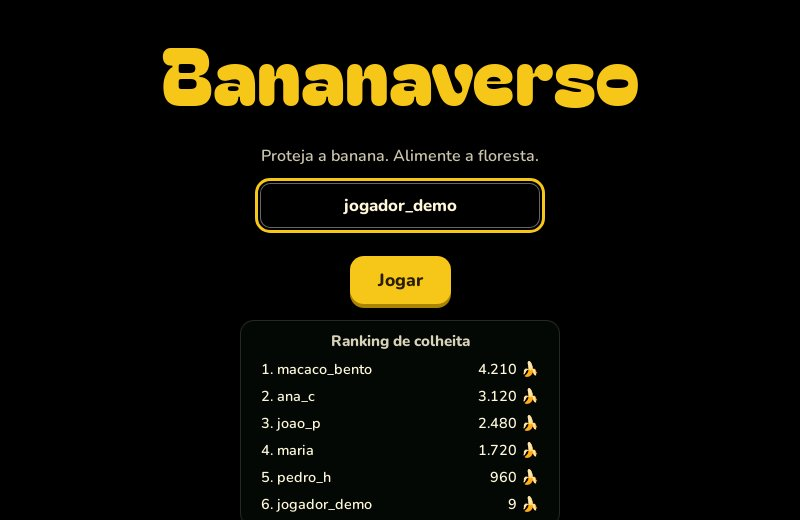
\includegraphics[width=0.66\linewidth]{titulo.jpg}
\caption{Tela inicial, com o campo de nome e o ranking global.}
\label{fig:titulo}
\end{figure}

\begin{figure}[H]
\centering
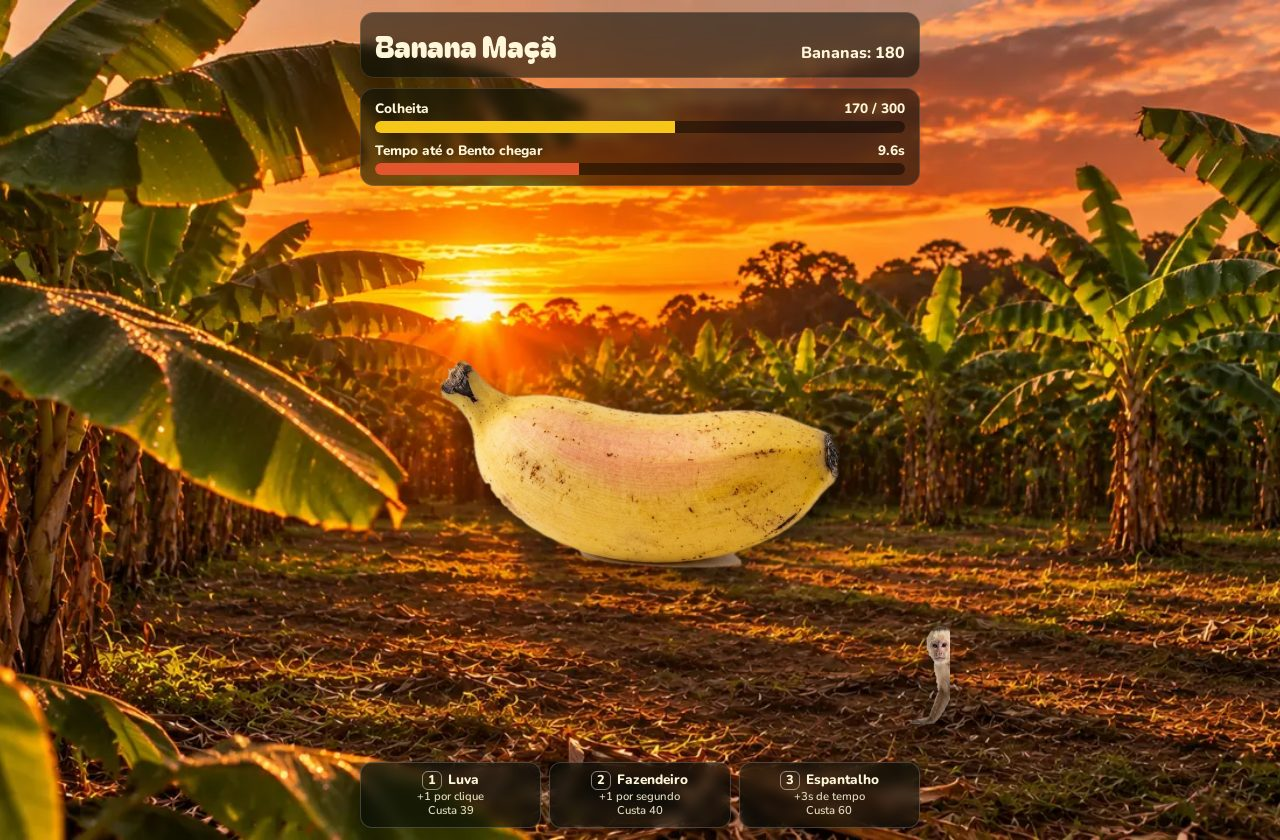
\includegraphics[width=0.66\linewidth]{jogo.jpg}
\caption{Partida em andamento na terceira fase (Banana Maçã).}
\label{fig:jogo}
\end{figure}

\begin{figure}[H]
\centering
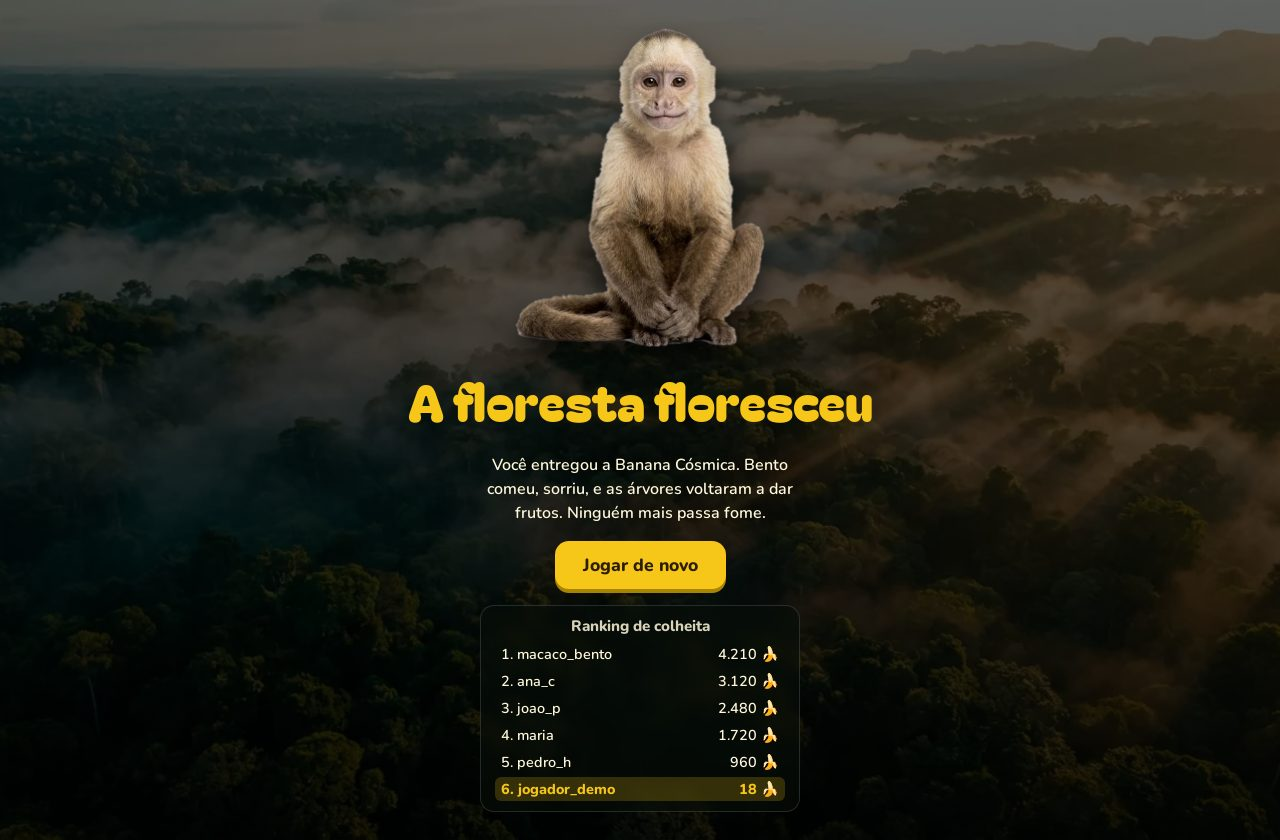
\includegraphics[width=0.66\linewidth]{vitoria.jpg}
\caption{Tela de vitória, com o ranking e o jogador destacado.}
\label{fig:vitoria}
\end{figure}

\subsection{Validação}

A aplicação foi validada de ponta a ponta com os três serviços em
execução. Todas as rotas foram exercitadas pelo nginx com o
\texttt{curl}, confirmando a soma dos incrementos, a ordem do ranking, a
recusa de valores acima do limite e de nomes inválidos (HTTP 422) e a
resposta 404 para jogadores inexistentes. Em seguida, um navegador
\emph{headless} (Playwright) percorreu a história, as cinco fases e a tela
de vitória, confirmando que as 22 imagens carregam, que nenhuma
requisição falha e que a colheita chega ao banco.

% =====================================================================
\section{Conclusão}\label{sec:conclusao}

O Bananaverso atende aos requisitos do projeto: é uma aplicação web
acessível pelo navegador, composta por três serviços em contêineres, dos
quais a API é de implementação própria. A separação entre servidor web,
API e banco, a comunicação apenas pela rede interna e a inicialização
controlada por \emph{healthchecks} reproduzem, em escala pequena, a forma
como aplicações são organizadas em nuvem.

Como trabalhos futuros, o grupo identifica: autenticação dos jogadores,
hoje identificados apenas pelo nome; validação no servidor de que a
colheita enviada é compatível com o tempo de jogo; e a implantação em um
provedor de nuvem, substituindo o banco em contêiner por um serviço
gerenciado.

% =====================================================================
\begin{thebibliography}{9}

\bibitem{nist}
Mell, P. and Grance, T. (2011).
\newblock The NIST definition of cloud computing.
\newblock Special Publication 800-145, National Institute of Standards and
  Technology.

\bibitem{merkel}
Merkel, D. (2014).
\newblock Docker: lightweight Linux containers for consistent development
  and deployment.
\newblock {\em Linux Journal}, 2014(239).

\bibitem{bernstein}
Bernstein, D. (2014).
\newblock Containers and cloud: from LXC to Docker to Kubernetes.
\newblock {\em IEEE Cloud Computing}, 1(3):81--84.

\bibitem{fielding}
Fielding, R. T. (2000).
\newblock {\em Architectural Styles and the Design of Network-based
  Software Architectures}.
\newblock PhD thesis, University of California, Irvine.

\bibitem{compose}
Docker Inc. (2026).
\newblock Docker Compose documentation.
\newblock \url{https://docs.docker.com/compose/}. Acesso em: nov. 2026.

\bibitem{fastapi}
FastAPI (2026).
\newblock FastAPI documentation.
\newblock \url{https://fastapi.tiangolo.com/}. Acesso em: nov. 2026.

\bibitem{psycopg}
Psycopg (2026).
\newblock Psycopg 3 documentation.
\newblock \url{https://www.psycopg.org/psycopg3/docs/}. Acesso em: nov. 2026.

\bibitem{nginx}
nginx (2026).
\newblock nginx documentation.
\newblock \url{https://nginx.org/en/docs/}. Acesso em: nov. 2026.

\end{thebibliography}

\end{document}
